\chapter{High rate software testing}
\section{Firmware-Based Data Acquisition}
The Mu2e Trigger and Data Acquisition (TDAQ) system collects digitized data from the Tracker, Calorimeter, Cosmic Ray Veto and Beam Monitoring components (Stopping Target Monitor and Extinction Monitor) and delivers that data to online and offline processing for analysis. It must merge data from $\sim$450 subsystems and apply filters to reduce data volume by a factor of 100 before storing it offline. It is also responsible for detector synchronization, control, monitoring and operator interfaces. The Mu2e DAQ system uses a $streaming$ readout technique, which means that all detector data from the experiment is digitized and zero-suppressed in their respective Front End Electronics (FEEs) before being transferred. This strategy results in a high data flow in the DAQ system while providing greater flexibility in data selection and analysis.
\subsection{Expected rate}
The data-taking periods will be divided in two modes: on-spill and off-spill. The on-spill mode covers periods when 8 GeV proton bunch are colliding the production target. The off-spill mode covers all other periods: between bunches, calibration periods, commissioning. 
Calling what is written in section XX, it is possible to estimate the on-spill event contribution:
\begin{itemize}
    \item 43.1ms (time of one spill)/ 1695ns(digitization time) = 25K pulses per spill
    \item 8(number of spills)*25K=200K on spill events /cycle
    \item 200K/ 1.4s(cycle time) = 145K ON Spill events/s
\end{itemize}
di questi 1.4s, 1.055s si riferisce all'offspill e 0.4s all'onspill.
Meanwhile, the off-spill event contribution is:
\begin{itemize}
    \item 145K ON Spill events/s*0.4s=58Kevents
    \item 55 K /1.4s= 41K off spill events per second per cycle
\end{itemize}
buffering: 0.4/1.4
\\
TOTAL INPUT: 186Kevents/s (Hz).
\\
INPUT EVENT SIZE:150KBytes/bunch(1695ns)=90GB/s
\\
buffering:0.4s(on spill)/1.4s(off spill)
\\
TOTAL: 90GB/s*0.4s(on spill)/1.4s(off spill)= 28GBytes/s
\\
online processing factor: 100(trigger that is after the farm manager and it is an approximation because it depends on the the input rate)
\\
TOTAL OUTPUT (that goes to boardreaders): 1.5kHz
\\
TOTAL: 1.5Kevents /s (Hz)*150KBytes/event=225MBytes/s
\\
The detector will generate $\sim$150 KB of zero-suppressed data per bunch (in un bunch ci sono 1695 ns), Section \ref{accel}, for an average data rate of $\sim$90 GB/s when beam is present. To reduce DAQ bandwidth requirements, this data is buffered in Readout
Controller (ROC) memory during the spill period and transmitted to the DAQ over the full supercycle for an average data rate of $\sim$28 GBytes/sec.

In Figure \ref{fig:linktodaq}, the general design of the Mu2e DAQ system is shown.
\begin{figure}[!h]
\centering
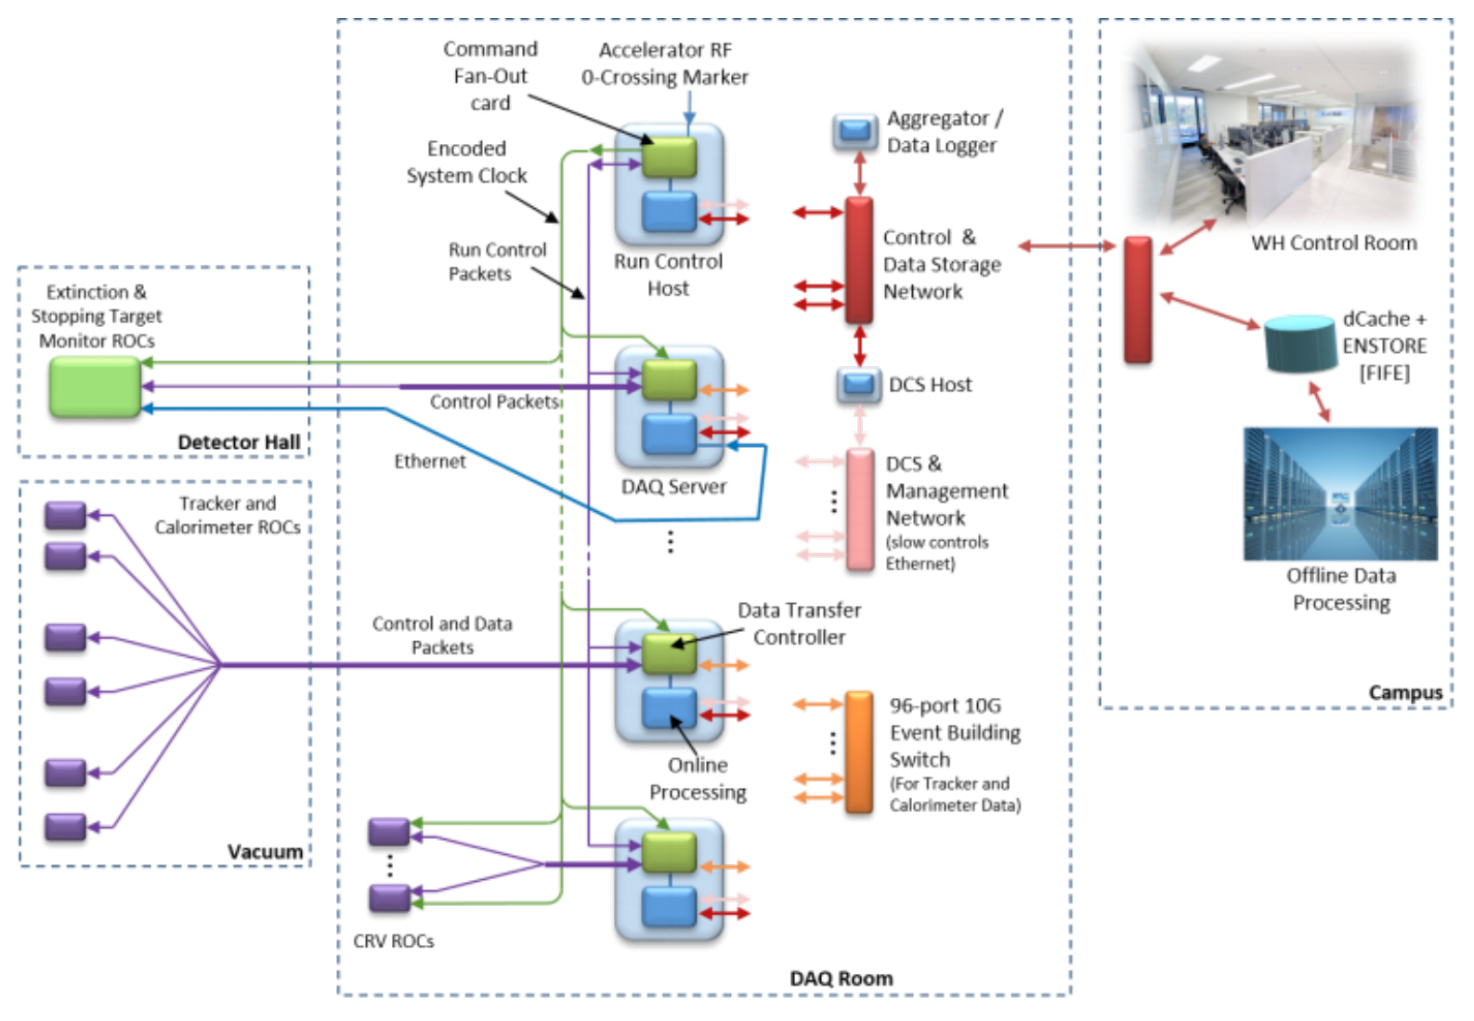
\includegraphics[width =\textwidth]{figures/png/Screenshot_20240206_144803.png}
\caption{Mu2e DAQ Architecture.}
\label{fig:linktodaq}
\end{figure}
The left blocks represent the Readout Controllers (ROCs) in different detectors. The center block houses the DAQ system's online components, which include the Run Control Host, 40 DAQ servers, the Detector Control System (DCS) and the Event Building Switch. The Run Control Host receives beam status and timing information from the Accelerator Controls network and operator commands from the remote control room. The Detector Control System (DCS) is the window onto the status and health of the Mu2e detector. The Event Building (EVB) function combines these subsets to form a complete detector data set for analysis by an online processor, Ref. \cite{bartoszek2015mu2e}. Event building is typically done in a switching network to sustain high rates. The right block houses the DAQ system's offline components, which are used for data storage and processing. During an active spill (the first approximately 43 ms of the 48 ms bunch extraction cycle outlined in Chapter \ref{accel}), the experiment receives RF Zero-Crossing Markers from the Accelerator that are synchronized to the 1695 ns proton pulse cycles (the event windows). Based on these markers, the Command Fan-Out (CFO) module within the Run Control Host generates a 40 MHz system clock and encodes Event Window Markers (EWMs) in the system clock to indicate the start of the event windows. The CFO then sends the encoded system clock, along with run control packets, to Data Transfer Controllers (DTCs) in the DAQ servers. The DTCs\footnote{The Mu2e Data Transfer Controller (DTC), Ref. \cite{ryan} takes data from various Read-Out Controllers and may conduct event construction and data preprocessing. The DTC module connects a maximum of six ROCs to the Trigger and Data Acquisition (TDAQ) servers, which execute the TDAQ online software framework.} then transfer the encoded clock to the detectors' ROCs, where the EWMs are recovered with fixed delay relative to the original RF Zero-Crossing Markers and used in the local ROCs to discriminate data acquired during consecutive event windows. The Tracker generates a DDR3 memory address at the beginning of each event window. The relevant memory area is designated to hold Tracker hits received during that event window. Data requests trigger data readouts from the ROCs to the DAQ system. The Data Requests are modifiable through the CFO as described by the Run Plan, although they are initially given to the Tracker and Calorimeter ROCs via the DTCs following each event window.

\subsection{TDAQ software: artdaq}





\subsubsection{Expected rate}





Each hit is composed of a data packet having a fixed length of 128 bits (16 bytes):
\begin{itemize}
    \item 16 bit header - it contains information as a packet header, a channel identifier to specify the channel so the ROC can assign the hit to a wire number and a packet checksum;
    \item 16 bit - TDC left straw end;
    \item 16 bit - TDC right straw end;
    \item 8$\times$10 bit ADC.
\end{itemize}
A packet of 128 bits can be transferred every 640 ns (200 Mbps).An additional 32
bits must be added as an end-of-file marker after the data $\mu$spill hit data is buffered.
The ROC-to-DAQ connection is made via fiber optic links arranged in rings, with multiple ROC per ring, as shown in Figure \ref{fig:linktodaq}. This is possible since a single optical link can handle 2.6 Gbps, while the ROC output is around 230 Mbps. This value comes from the fact that the highest rate for any 4 straws group (corresponding to one digitizer data line to the ROC) is 240 kHz or 30 Mbps (at 128 bits/hit) and the Main Injector supplies Mu2e beam only 32\% of the time. The ROC monitors slow control variables and controls panel operations too.


XXXXXXXXX: mettere le caratteristiche di Ref. \cite{vadi}  ?????
